%% ID: fairground_ride
%% TITLE: A Fairground Ride
%% TYPE: question
%% QUESTIONTYPE: symbolic
%% CONCEPTS: angular_circular, friction, vectors, resolving_vectors
%% LEVEL: 4
%% TOPIC: mechanics/circular
%% ORDER: 10

\begin{problem}[Nicki_Suggestion_Fair]
{\exposition{A fairground ride consists of a rough cylinder that rotates about a vertical axis through its centre. Once people are inside and the cylinder is rotating fast enough the floor is removed but the thrillseekers do not fall down.} The coefficient of friction between the people and the cylinders is \vari{\mu} and the cylinder has radius \vari{R}. \question{What is the minimum angular speed at which it needs to rotate for the ride to be safe?}
}
{\stress{Created for the Rutherford School Physics Project by NHB and ES}}
{The forces acting on someone on the ride are shown in Figure \ref{fig:CircularMotion_h}:
\begin{figure}[h]
\centering
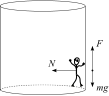
\includegraphics[width=5cm]{../../../figures/CircularMotion_h.eps}
\caption{}
\label{fig:CircularMotion_h}
\end{figure}
The reaction force \vari{\vtr{N}} from the wall provides the centripetal force so
\begin{equation*}
N=mR\omega^2
\end{equation*}
for mass \vari{m}, angular speed \vari{\omega}. In order for the rider not to fall, the magnitude of the frictional force \valuedef{F}{\mu N}{} must balance the weight of magnitude \vari{mg}. Therefore
\begin{align*}
F=\mu N=mg \\
\Rightarrow \mu mR\omega^2=mg \\
\Rightarrow \omega^2=\frac{g}{\mu R}
\end{align*}

The requirement is 
\begin{equation*}
\omega\ge\sqrt{\frac{g}{\mu R}}
\end{equation*}

\answer{The minimum angular speed needed for the ride to be safe is \valuedef{\omega}{\sqrt{\frac{g}{\mu R}}}{}.}
}
\end{problem}